\documentclass[UTF8]{article}
\usepackage{xeCJK}
\setCJKmainfont{Songti SC}       % 宋体

\usepackage{booktabs}
\usepackage{siunitx}
\sisetup{table-number-alignment = center, round-mode=places, round-precision=3}

\usepackage{longtable}
\usepackage{booktabs}
\usepackage{siunitx}
\usepackage{caption}

\usepackage{minted}
\usepackage{listings}
\usepackage{xcolor}

\lstset{
  language=Matlab,
  basicstyle=\ttfamily\small,    % 代码字体
  numbers=left,                  % 行号位置
  numberstyle=\tiny,             % 行号字体
  keywordstyle=\color{blue},     % 关键字颜色
  commentstyle=\color{gray},     % 注释颜色
  stringstyle=\color{red},       % 字符串颜色
  frame=single,                  % 边框
  breaklines=true,               % 自动换行
  showstringspaces=false,        % 不显示空格
  tabsize=4,                     % Tab宽度
  captionpos=b                   % 标题位置 bottom
}


\usepackage{booktabs}
\usepackage{tabularx}
\usepackage{array}
\usepackage{threeparttable}

\usepackage{graphicx}
\usepackage{subfigure}  % 或者叫 subcaption,二选一
\usepackage{caption}

\usepackage{ctex}
\usepackage{graphicx}
\usepackage{amsmath,amssymb}
\usepackage{siunitx}
\usepackage{textcomp}
\usepackage{float}
\usepackage[a4paper,margin=2cm]{geometry}
\sisetup{per-mode=symbol}
\usepackage{tikz}
\usetikzlibrary{arrows.meta,positioning,fit,shapes,calc}
\XeTeXlinebreaklocale "zh"
\XeTeXlinebreakskip = 0pt plus 1pt

\begin{document}
% === 标题部分 ===
\begin{center}
    {\LARGE\bfseries 用 SSH 分析西北太平洋海面高度的气候态与季节变化}\\[1.2em]  % 标题(加粗 + 空行)
    {\large 报告人:XX \quad 学号:20XX8345XXXX}\\[0.5em]  % 居中放置人名与学号
\end{center}

\section{实习目的}
复习MATLAB的基本数据读取和绘图功能,了解m\_map工具包的应用

深化理解海面动力高度在全球的时空分布特征和物理意义
\section{实习资料}
Matlab 2025b软件和sshg.2007.nc与sshg.2017.nc

\section{主要方法}
本研究使用的sshg.2007.nc与sshg.2017.nc文件均为NetCDF格式的海面高度(Sea Surface Height,SSH)栅格数据文件,文件格式为classic类型。两个文件结构一致,主要存储了2007年与2017年全球(或区域)范围内的逐月海面高度异常场(Sea Surface Height Gridded,SSHG),是进行海洋气候态、年际变化及风场–海平面耦合分析的重要基础数据。
文件包含三个主要维度(经度、纬度、时间),六个变量以及十三个全局属性。主要数据变量为sshg,其余变量包括经纬度与时间坐标信息。

\subsection{数据结构与变量说明}
\subsubsection{维度信息}
\begin{table}[htbp]
\centering
\caption{SSH 数据维度说明}
\begin{threeparttable}
\begin{tabularx}{0.95\textwidth}{
  >{\centering\arraybackslash}m{2.3cm}  % 列1
  >{\centering\arraybackslash}m{2.3cm}  % 列2
  >{\centering\arraybackslash}m{2.3cm}  % 列3
  >{\centering\arraybackslash}X         % 列4
}
\toprule
\textbf{维度名称} & \textbf{含义} & \textbf{大小} & \textbf{说明} \\
\midrule
lon  & 经度 & 360 & 从西向东均匀分布 \\
lat  & 纬度 & 418 & 从南到北均匀分布 \\
time & 时间 & 12  & 表示 12 个月的月平均值 \\
\bottomrule
\end{tabularx}
\end{threeparttable}
\end{table}

\subsubsection{变量信息}
\begin{table}[H]
\centering
\caption{SSH 文件变量信息表}
\begin{threeparttable}
\begin{tabularx}{0.95\textwidth}{
  >{\centering\arraybackslash}m{2.3cm}  % 与表1完全一致
  >{\centering\arraybackslash}m{2.3cm}
  >{\centering\arraybackslash}m{2.3cm}
  >{\centering\arraybackslash}X
}
\toprule
\textbf{变量名} & \textbf{数据类型} & \textbf{维度} & \textbf{说明} \\
\midrule
lon      & double & [360]             & 经度(单位:$^\circ$E) \\
lat      & double & [418]             & 纬度(单位:$^\circ$N) \\
time     & double & [12]              & 时间步长,对应 1–12 月 \\
date     & char   & [12]              & 日期字符串(如“2007–01”) \\
timePlot & double & [12]              & 用于绘图的时间辅助变量 \\
sshg     & int16  & [360$\times$418$\times$12] & 海面高度异常主变量 \\
\bottomrule
\end{tabularx}
\end{threeparttable}
\end{table}
\subsubsection{主要变量 SSH 描述}
SSH 是文件的核心变量,表示在指定经纬度与月份下的海面高度异常值。其维度顺序为 [lon, lat, time],即经度×纬度×时间。
数据类型为int16,一般需要在读取后转换为 double 类型以便计算。SSH 的物理意义为:海面相对于多年平均海平面的高度偏差,反映海洋动力过程、热胀冷缩效应以及环流系统的变化特征。
时间维度的 12 个样本分别对应当年的 1 月至 12 月。

\begin{figure}[H]
\centering
\subfigure[2007 年 SSH 年平均海面高度分布]{
    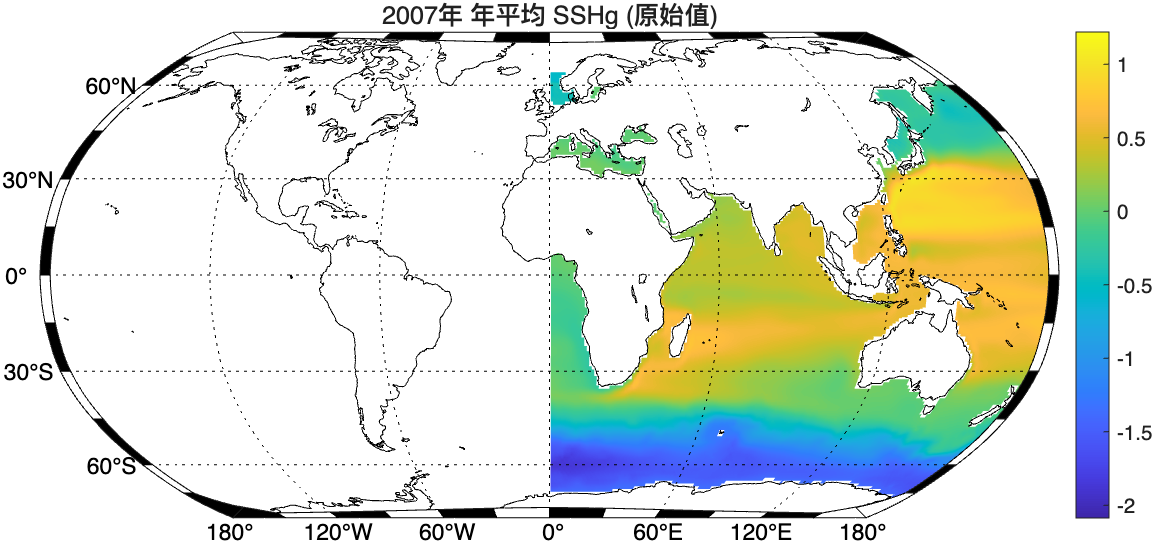
\includegraphics[width=0.45\textwidth]{Figure_2 2007.png}
}
\subfigure[2017 年 SSH 年平均海面高度分布]{
    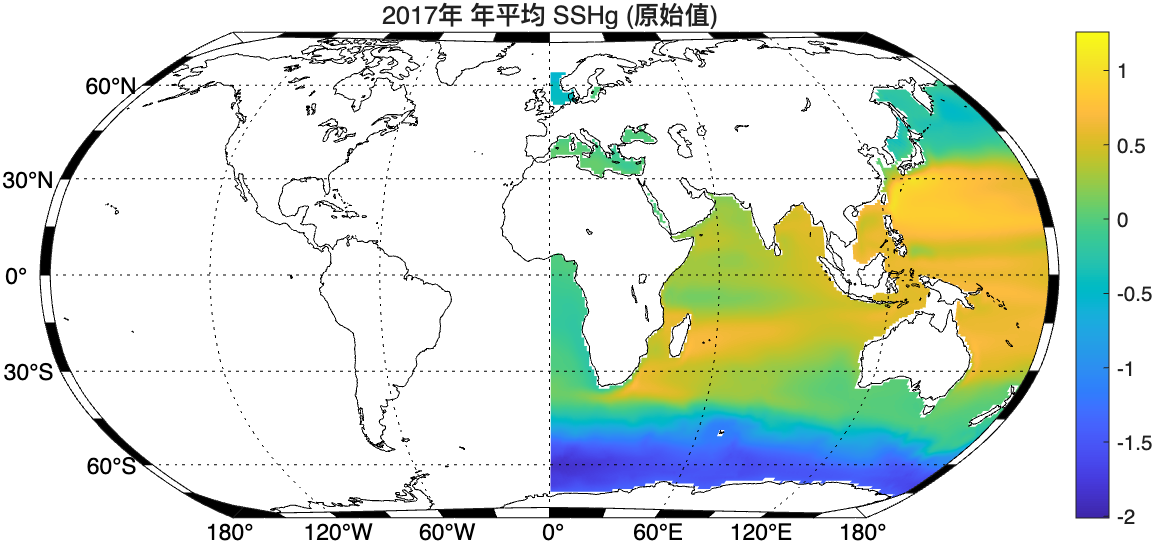
\includegraphics[width=0.45\textwidth]{Figure_2.png}
}
\caption{2007 年与 2017 年 SSH 年平均海面高度对比图}
\label{fig:2007 年与 2017 年 SSH 年平均海面高度对比图}
\end{figure}

\begin{figure}[H]
\centering
\subfigure[2007 年 SSH 月平均海面高度分布]{
    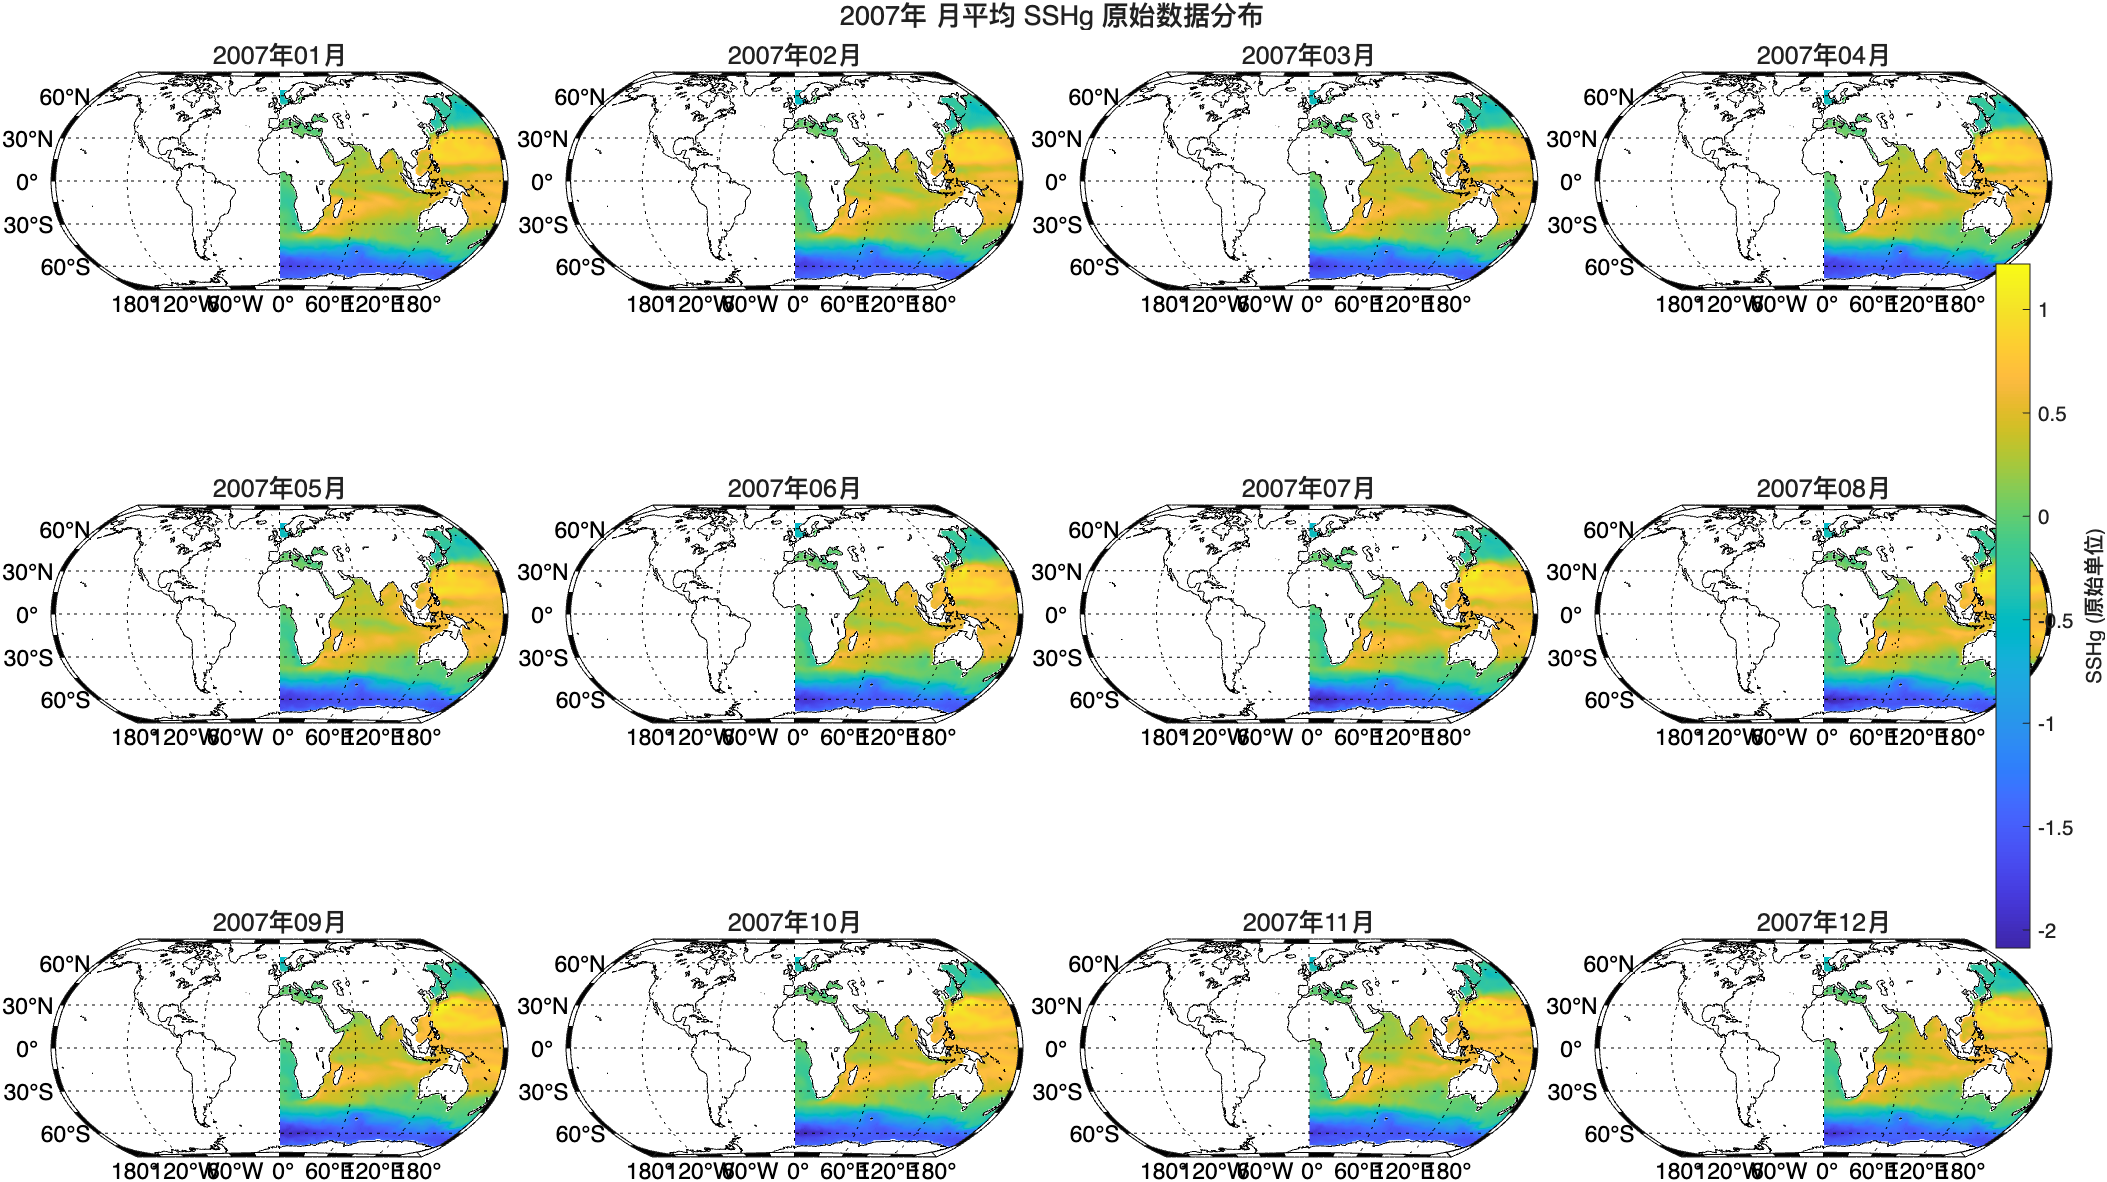
\includegraphics[width=0.68\textwidth]{Figure_1 2007.png}
}
\subfigure[2017 年 SSH 月平均海面高度分布]{
    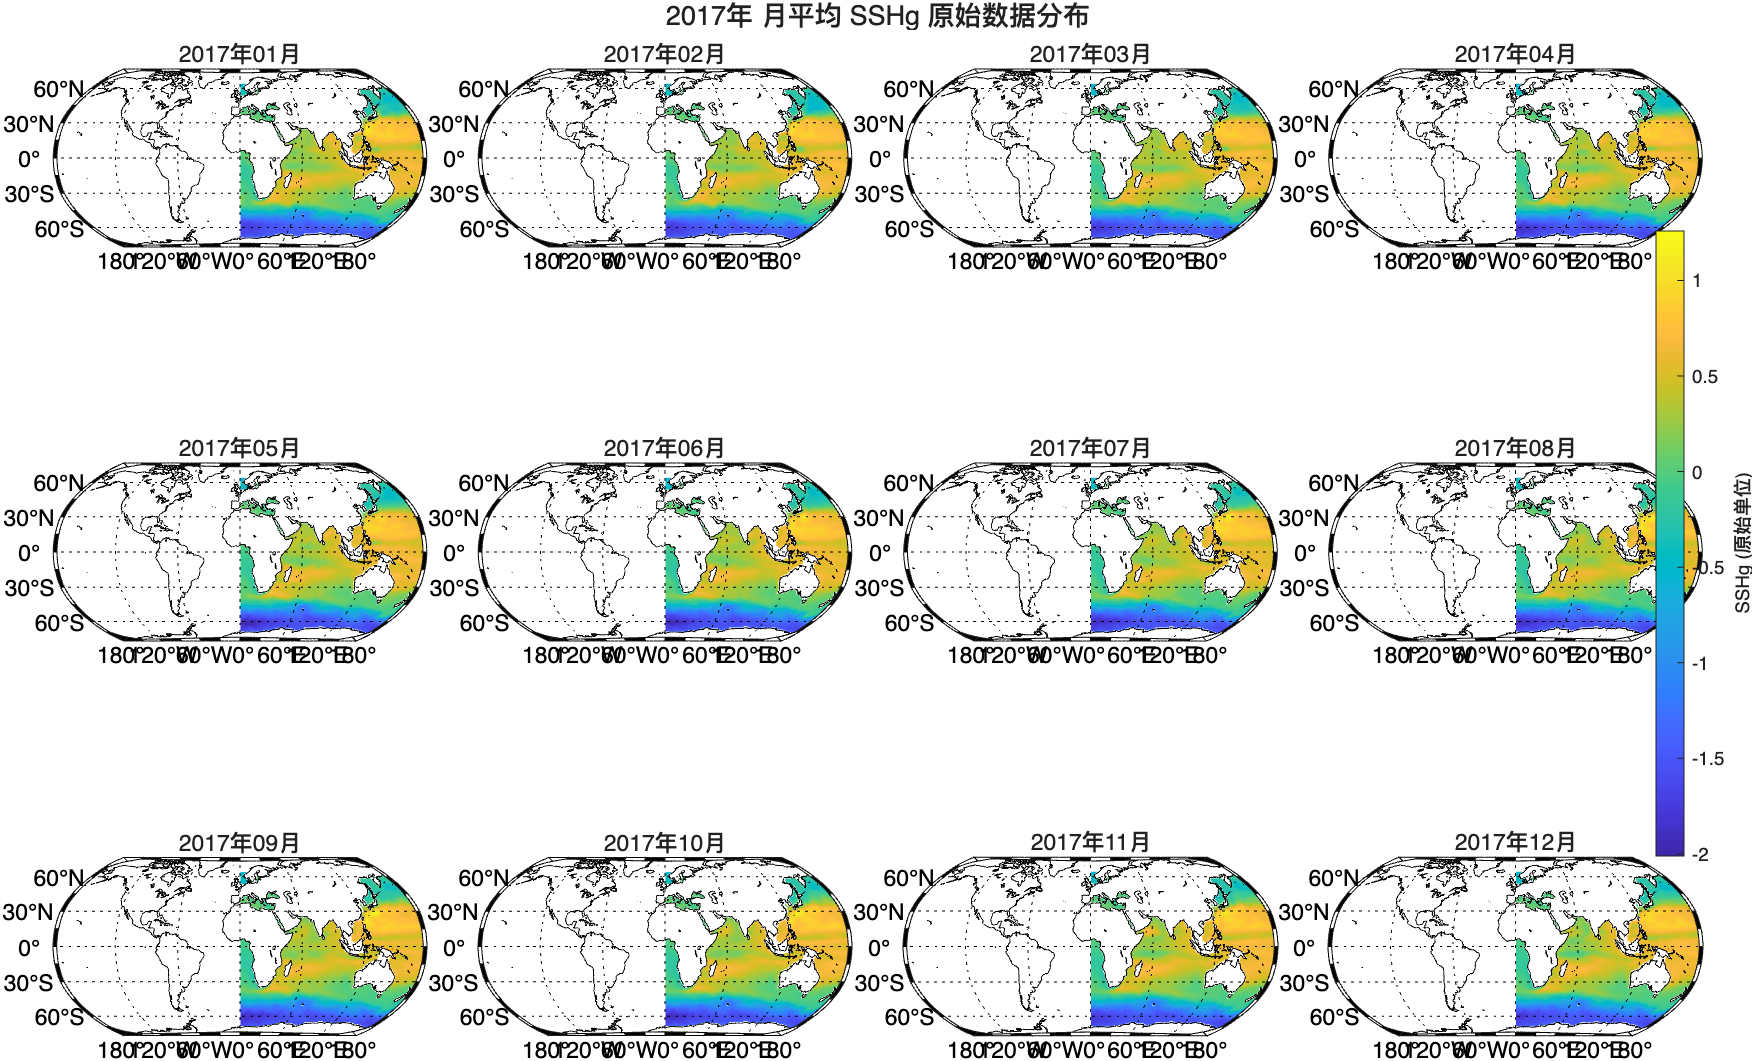
\includegraphics[width=0.68\textwidth]{Figure_1.png}
}
\caption{2007 年与 2017 年 SSH 月平均海面高度对比图}
\label{fig:2007 年与 2017 年 SSH 月平均海面高度对比图}
\end{figure}

\begin{figure}[H]
\centering
\subfigure[2007 年 SSH 空间平均的时间序列图]{
    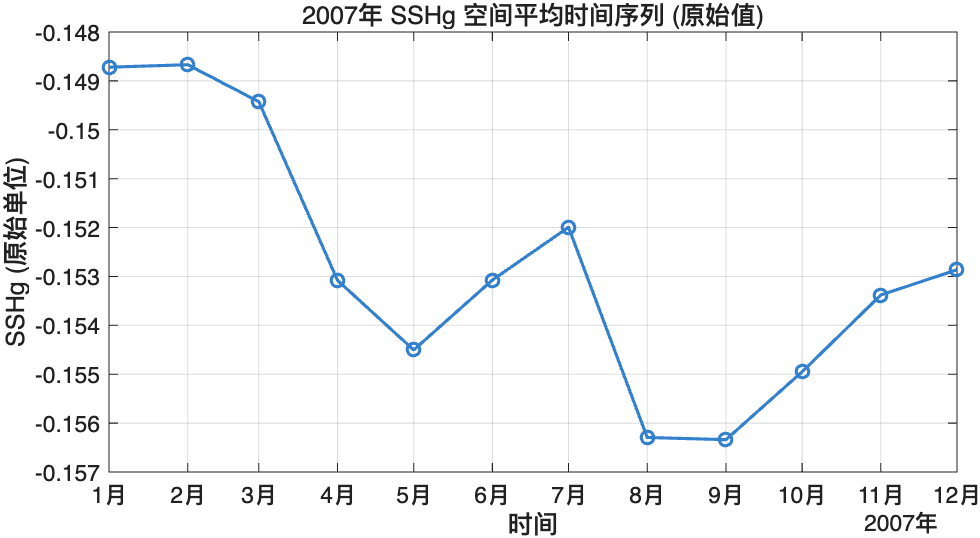
\includegraphics[width=0.45\textwidth]{Figure_3 2007.png}
}
\subfigure[2017 年 SSH 空间平均的时间序列图]{
    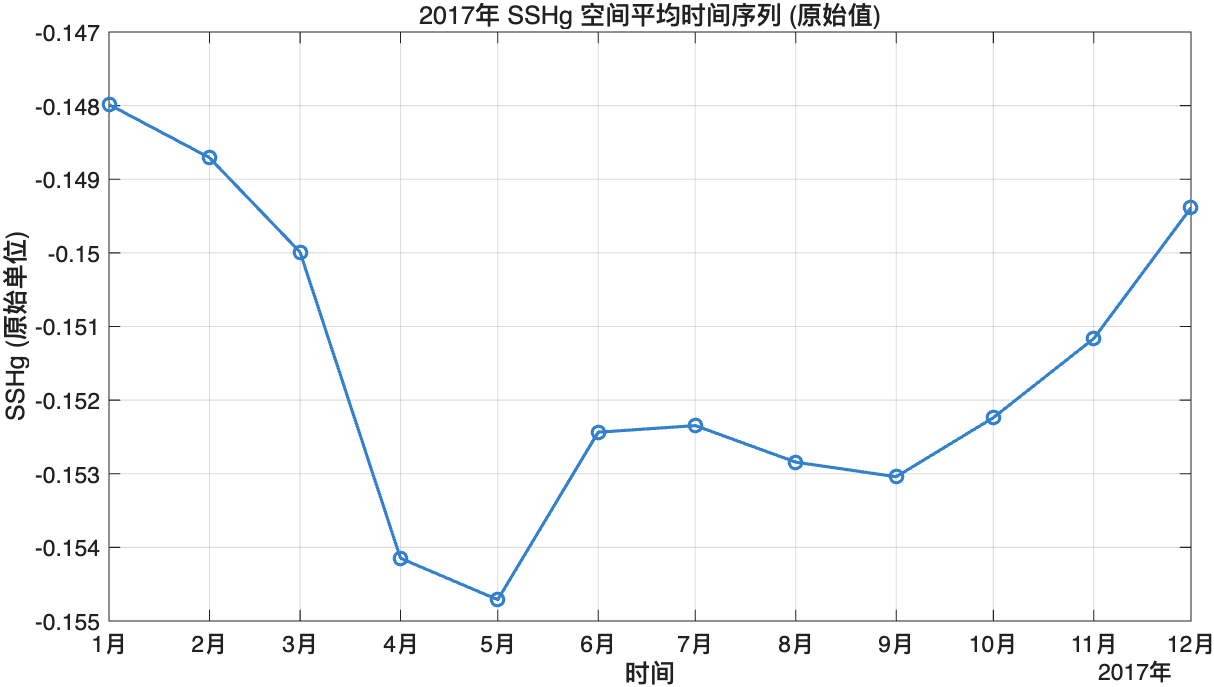
\includegraphics[width=0.45\textwidth]{Figure_3.png}
}
\caption{2007 年与 2017 年 SSH 月空间平均的时间序列图}
\label{fig:2007 年与 2017 年 SSH 月空间平均的时间序列图}
\end{figure}






\section{主要内容}
\subsection{研究区与数据处理}
研究区选取为西北太平洋 $120^\circ\!-\!160^\circ\mathrm{E},\,10^\circ\!-\!40^\circ\mathrm{N}$区域。
覆盖黑潮主流/延伸体(KE)与其南侧的副热带环流内海域,是西北太平洋上层环流的动力核心区。北界未超过 $40^\circ\mathrm{N}$,避开强冬季深对流与近岸陆架过程的主导影响、南界到 $10^\circ\mathrm{N}$ 足以包含副热带环流内的高 SSH 脊线。
保证环流信号清晰。数据处理使用月平均SSHg构建四季合成与年平均。
统一色标(同一图组内四季/两年一致),保证横向可比性。
计算研究区内面积加权区域平均得到1–12 月月循环。


\subsection{气候态空间分布(年平均与四季平均)}
\subsubsection{年平均基本态}
研究区呈现典型副热带环流的海面高度场,南部($15^\circ\!-\!25^\circ\mathrm{N}$)高、北部($30^\circ\!-\!40^\circ\mathrm{N}$)低。
黑潮/KE 在 $30^\circ\!-\!35^\circ\mathrm{N},\,135^\circ\!-\!155^\circ\mathrm{E}$ 一带,SSHg 等值线密集,呈现显著的带状梯度带,对应 KE 主轴位置与强东向流区。
可见2007 年的 SSH 整体偏高于 2017 年,尤其在 $20^\circ\!-\!30^\circ\mathrm{N},\,135^\circ\!-\!150^\circ\mathrm{E}$ 的副热带内部与 KE 南侧。

\begin{figure}[H]
    \centering
    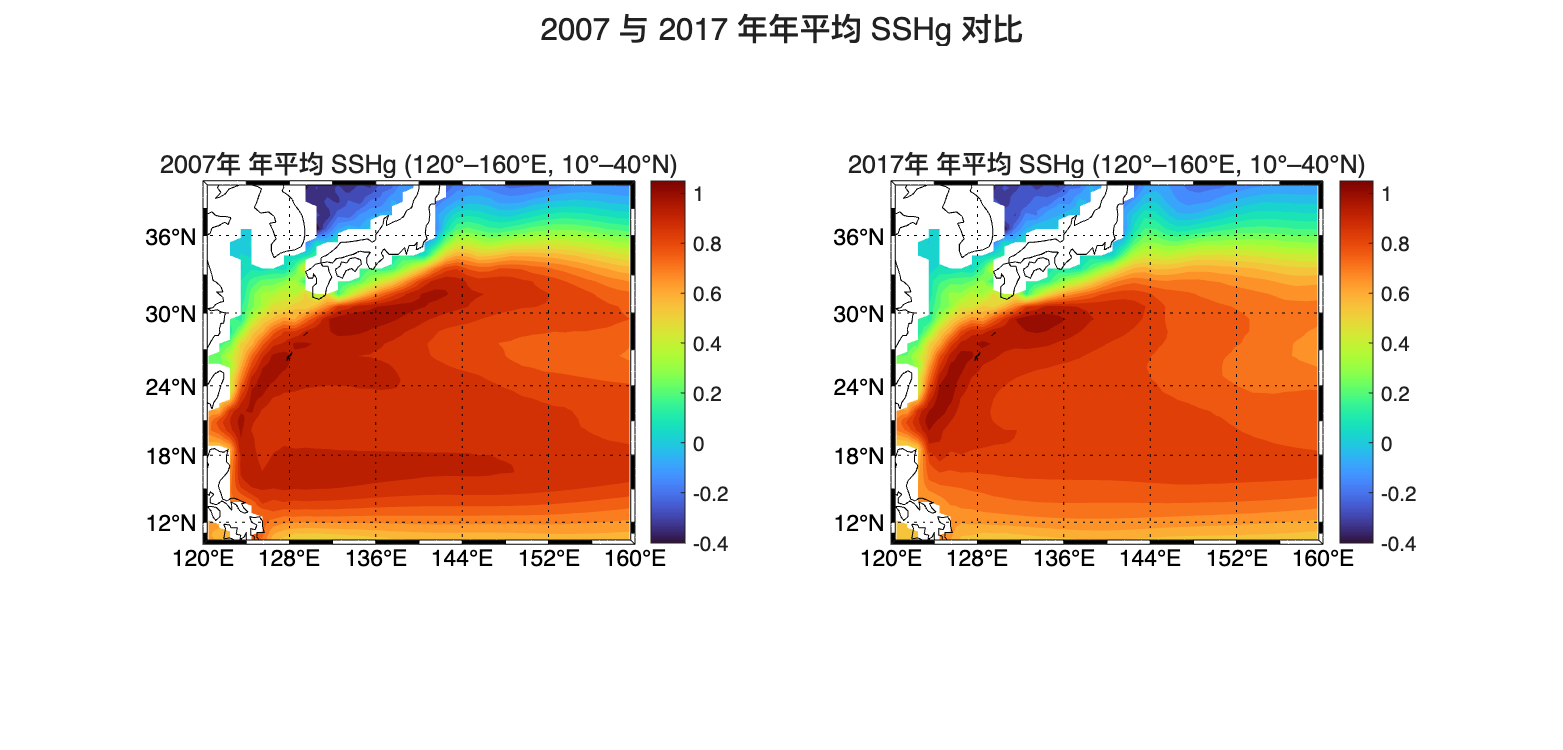
\includegraphics[width=0.95\textwidth]{SSHg_Annual_2007vs2017.png}
    \caption{2007 年与 2017 年年平均 SSHg 对比}
    \label{fig:sshg_annual}
\end{figure}

\subsubsection{四季平均}
\paragraph{冬季(DJF)}北部($30^\circ\!-\!40^\circ\mathrm{N}$)梯度最陡,KE 带状结构最清晰;2007 年相对 2017 年高值区更向西南扩展,指示该年冬季副热带环流/KE 势能更强。
\begin{figure}[H]
    \centering
    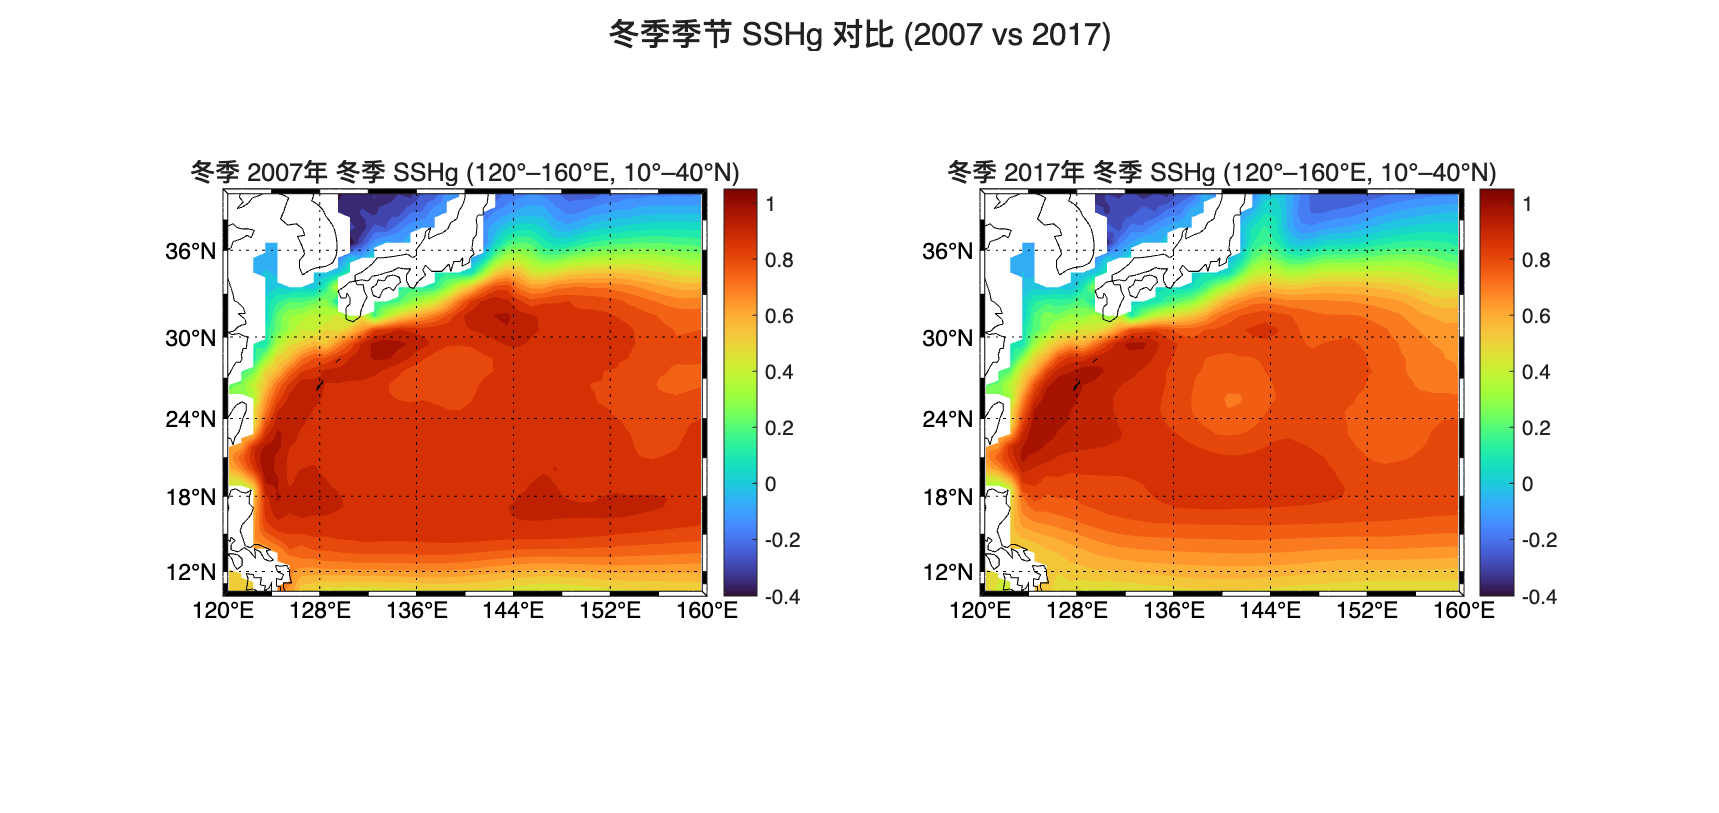
\includegraphics[width=0.95\textwidth]{SSHg_DJF_2007vs2017.png}
    \caption{冬季季节 SSH 对比(2007 vs 2017)}
    \label{fig:sshg_djf}
\end{figure}

\paragraph{春季(MAM)}整体 SSH 开始回升,梯度仍然较强但较冬季有所缓和。2007 年的高 SSH 带仍明显强于2017 年。
\begin{figure}[H]
    \centering
    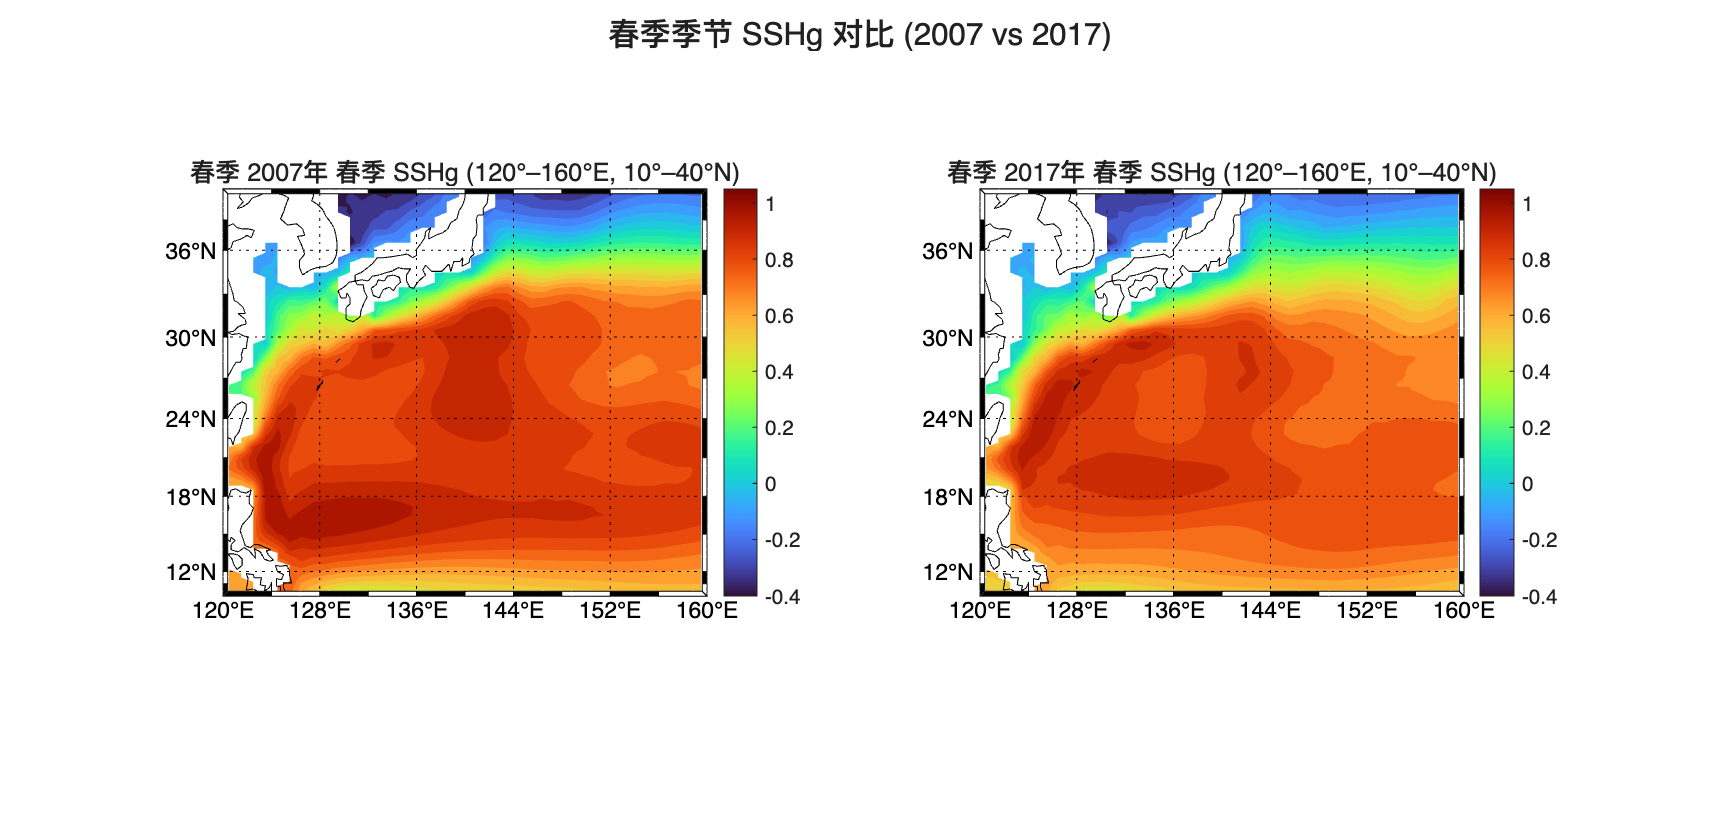
\includegraphics[width=0.95\textwidth]{SSHg_MAM_2007vs2017.png}
    \caption{春季季节 SSH 对比(2007 vs 2017)}
    \label{fig:sshg_mam}
\end{figure}

\paragraph{夏季(JJA)}南侧高值明显增强,高 SSH 区北伸,但纬向梯度较冬春弱。2007 年在 $25^\circ\!-\!33^\circ\mathrm{N}$ 的高值范围仍较 2017 年广。
\begin{figure}[H]
    \centering
    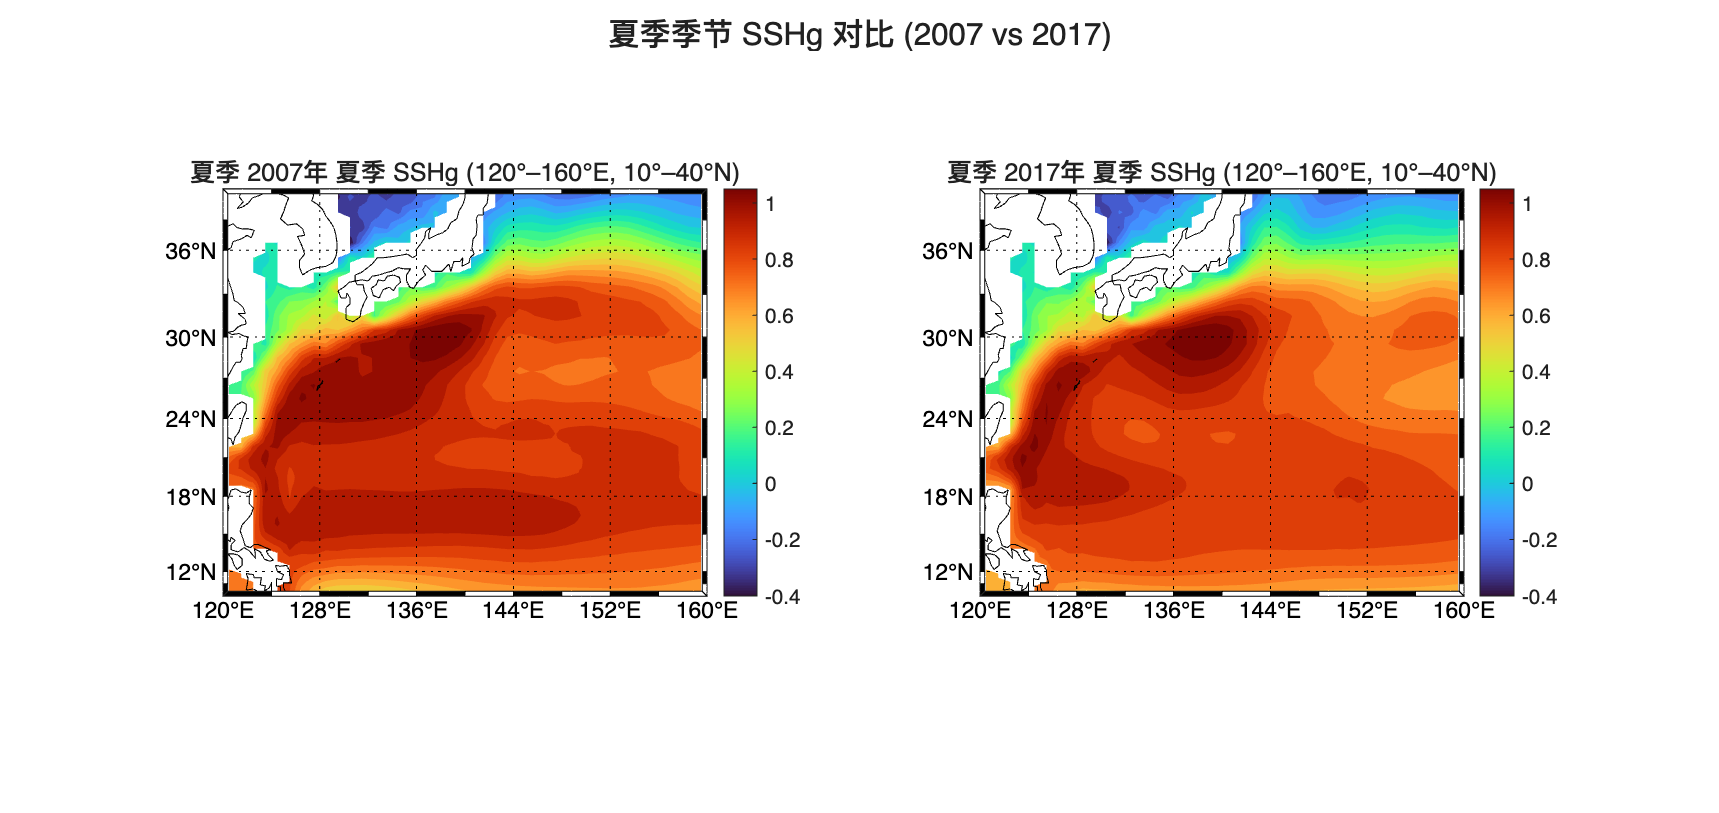
\includegraphics[width=0.95\textwidth]{SSHg_JJA_2007vs2017.png}
    \caption{夏季季节 SSH 对比(2007 vs 2017)}
    \label{fig:sshg_jja}
\end{figure}


\paragraph{秋季(SON)}仍维持较高 SSH 背景场,北部渐转弱、进入冬季态过渡。两年差异继续存在,2007 年偏高的格局保持。
\begin{figure}[H]
    \centering
    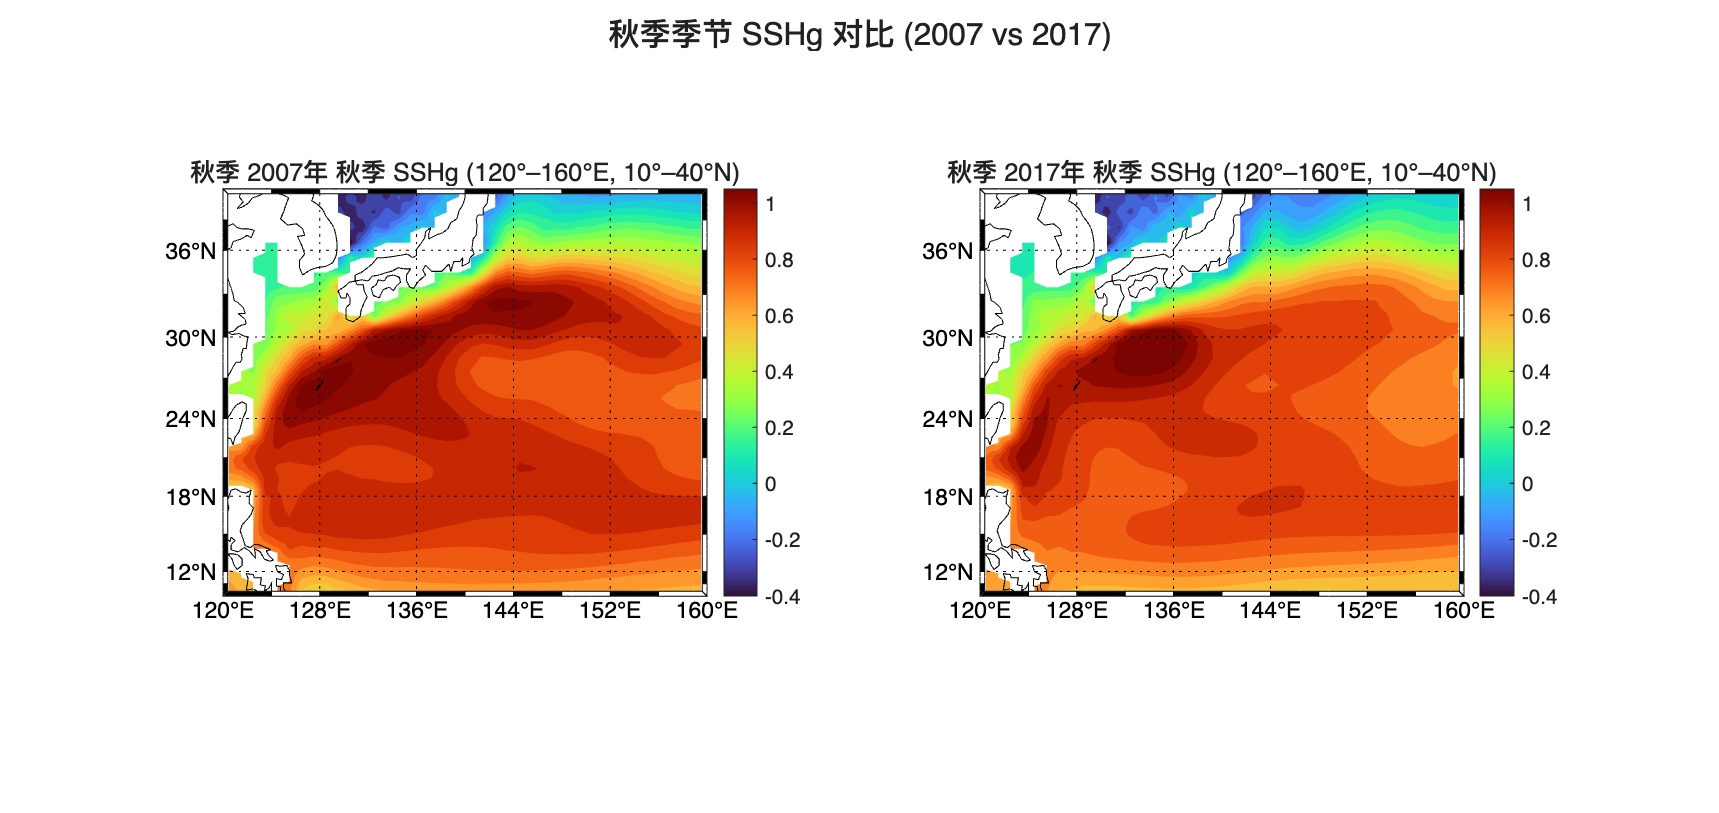
\includegraphics[width=1\textwidth]{SSHg_SON_2007vs2017.png}
    \caption{秋季季节 SSH 对比(2007 vs 2017)}
    \label{fig:sshg_son}
\end{figure}

\subsection{区域平均月循环(2007 vs 2017)}
季节上相位一致,两年均呈“冬季低、夏末—初秋高”的单峰型年循环。
年际幅度与水平上,
2007 年整体高于 2017 年。从曲线读数看,全年差值约 $0.05–0.08$,
最小值出现在 2–3 月($2007 \approx 0.65$、$2017 \approx 0.59$ 附近),
峰值出现在 8–9 月($2007 \approx 0.75–0.76、2017 \approx 0.69–0.70$),两年峰—谷幅度均约 $0.10±0.02$,2017 的振幅略小。
物理解释为区域平均 SSH 的年循环主要由热胀冷缩(海洋热含量)的季节变化与风应力涡度季节摆动共同控制。
\begin{figure}[H]
    \centering
    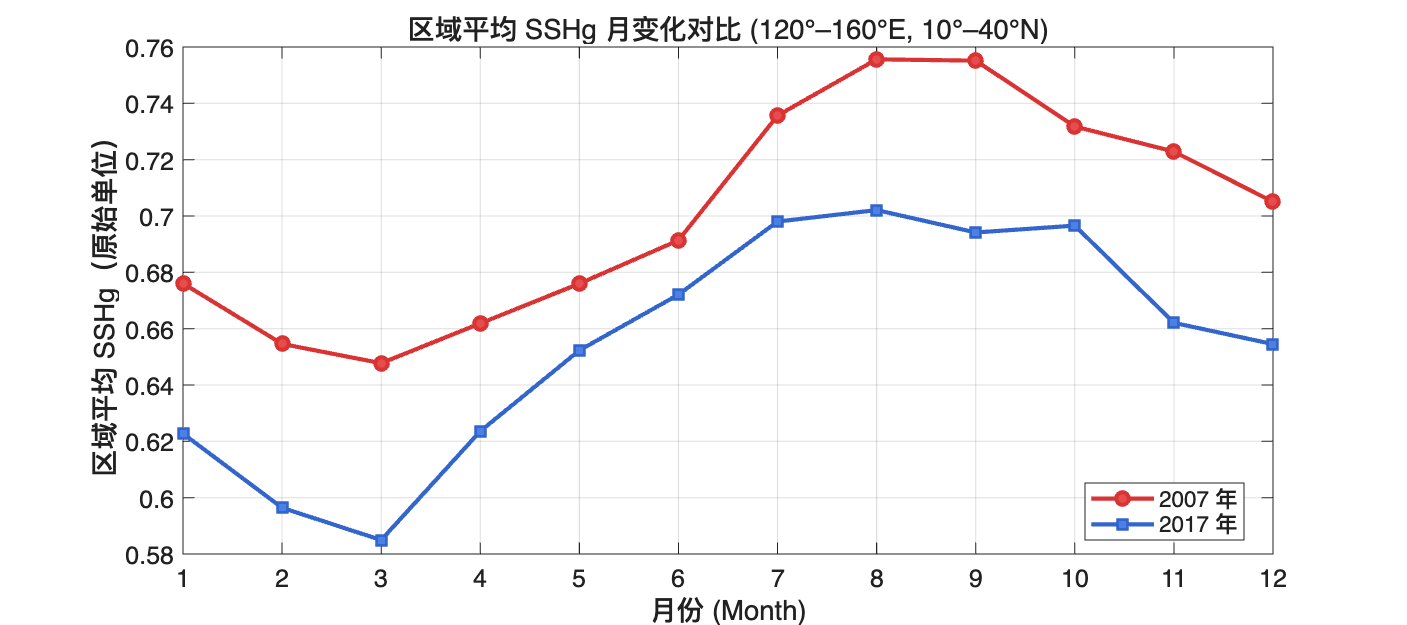
\includegraphics[width=0.85\textwidth]{SSHg_RegionalMean_TS_2007vs2017.png}
    \caption{区域平均 SSH 月变化对比($120°–160°E,10°–40°N$)。}
    \label{fig:SSH_ts}
\end{figure}





\section{实习小结}
本次实习通过对 2007 年与 2017 年西北太平洋海面高度(SSH)资料的对比分析,
系统复习了 MATLAB 的 NetCDF 数据读取、M\_Map 地图绘制及图像批处理方法。
通过编写自动化脚本,成功实现了四季平均、年平均以及区域平均时间序列的计算与可视化。

结果显示,研究区(120°–160°E,10°–40°N)具有典型的副热带环流结构:
南高北低,黑潮及其延伸体(Kuroshio Extension, KE)对应明显的 SSH 梯度带。
年际对比发现,2007 年的 SSHg 整体高于 2017 年,
尤其在 20°–30°N、135°–150°E 区域,表明该时期副热带环流较强、海洋热含量较高。
从年循环特征来看,两年均呈现“冬季低、夏秋高”的单峰型变化,
但 2017 年整体偏低且振幅略小,说明近十年间该区域可能存在热膨胀减弱
或风应力涡度调整等动力差异。

本次实验不仅加深了对 SSHg 数据物理意义的理解,
也提升了利用 MATLAB 进行海洋网格数据处理与空间可视化的能力,
为后续进行海洋气候态、黑潮变异及 ENSO 相关研究奠定了数据与方法基础。


\begin{thebibliography}{99}
\bibitem{Gill1982}
Gill, A. E. (1982).
\textit{Atmosphere–Ocean Dynamics}.
Academic Press, London.

\bibitem{Chelton1996}
Chelton, D. B., \& Schlax, M. G. (1996).
Global observations of oceanic Rossby waves.
\textit{Science}, \textit{272}(5259), 234–238.

\bibitem{Wunsch1998}
Wunsch, C., \& Stammer, D. (1998).
Satellite altimetry, the marine geoid, and the oceanic general circulation.
\textit{Annual Review of Earth and Planetary Sciences}, \textit{26}, 219–253.

\bibitem{Stammer1997}
Stammer, D. (1997).
Global characteristics of ocean variability estimated from regional TOPEX/Poseidon altimeter measurements.
\textit{Journal of Physical Oceanography}, \textit{27}(8), 1743–1769.

\bibitem{NOAA2024}
National Centers for Environmental Information (NCEI). (2024).
\textit{GODAS (Global Ocean Data Assimilation System) Sea Surface Height Data}.
NOAA, U.S. Department of Commerce.

\bibitem{Mathworks2025}
The MathWorks, Inc. (2025).
\textit{MATLAB R2025b Documentation}.
Natick, Massachusetts, USA.

\bibitem{OpenAI2025}
OpenAI. (2025).
\textit{ChatGPT (GPT-5) Technical Assistance Platform}.
OpenAI, San Francisco, CA, USA.

\end{thebibliography}


\section*{附录}
\subsection*{附录一}
\begin{minted}[fontsize=\small, frame=lines, linenos, breaklines]{matlab}
clear; clc; close all;

years = [2007, 2017];
basePath = '/Users/macbookair15/Desktop/海洋气象学/m_map/';
lonlim = [-180 180];
latlim = [-80 80];
cmap = parula(200);

for y = years
    fprintf('\n=============================\n');
    fprintf('  处理年份: %d\n', y);
    fprintf('=============================\n');

    fname = fullfile(basePath, sprintf('sshg.%d.nc', y));

    info = ncinfo(fname);
    disp('文件包含的变量:');
    disp({info.Variables.Name}');

    lon  = ncread(fname, 'lon');
    lat  = ncread(fname, 'lat');
    time = ncread(fname, 'time');
    sshg = ncread(fname, 'sshg');

    [nlat, nlon, ntime] = size(sshg);
    fprintf('SSHg 数据维度: %d×%d×%d (lat×lon×time)\n', nlat, nlon, ntime);

    minSSH = min(sshg(:));
    maxSSH = max(sshg(:));
    meanSSH = mean(double(sshg(:)), 'omitnan');
    fprintf('原始SSHg范围: %d ~ %d (平均值 = %.2f)\n', minSSH, maxSSH, meanSSH);

    %% === 时间变量转日期 ===
    refDate = datetime(1800,1,1,0,0,0);
    time_dt = refDate + days(time);

    %% === 绘制12个月平均图 ===
    clim = [double(minSSH) double(maxSSH)];

    figure('Name', sprintf('%d_Monthly', y), 'Position',[100 100 1200 800]);
    tiledlayout(3,4,'Padding','compact','TileSpacing','compact');
    for k = 1:ntime
        nexttile;
        m_proj('robinson','lon',lonlim,'lat',latlim);
        m_pcolor(lon, lat, double(sshg(:,:,k))); shading interp;
        m_coast('color','k');
        m_grid('box','fancy','tickdir','in');
        title(datestr(time_dt(k),'yyyy年mm月'));
        caxis(clim); colormap(cmap);
    end
    cb = colorbar('Position',[0.92 0.25 0.015 0.5]);
    cb.Label.String = 'SSHg (原始单位)';
    sgtitle(sprintf('%d年 月平均 SSHg 原始数据分布', y));

    %% === 年平均图 ===
    sshg_year = mean(double(sshg),3,'omitnan');
    figure('Name', sprintf('%d_AnnualMean', y), 'Position',[200 200 900 450]);
    m_proj('robinson','lon',lonlim,'lat',latlim);
    m_pcolor(lon, lat, sshg_year); shading interp;
    m_coast('color','k'); m_grid('box','fancy','tickdir','in');
    colorbar; colormap(cmap);
    caxis(clim);
    title(sprintf('%d年 年平均 SSHg (原始值)', y));

    %% === 空间平均时间序列 ===
    sshg_mean_time = squeeze(mean(double(sshg), [1 2], 'omitnan'));
    figure('Name', sprintf('%d_MeanTimeSeries', y), 'Position',[200 200 700 350]);
    plot(time_dt, sshg_mean_time, '-o', 'LineWidth',1.5, 'Color',[0.2 0.5 0.8]);
    xlabel('时间'); ylabel('SSHg (原始单位)');
    title(sprintf('%d年 SSHg 空间平均时间序列 (原始值)', y));
    grid on;
end
\end{minted}

\subsection*{附录二}
\begin{minted}[fontsize=\small, frame=lines, linenos, breaklines]{matlab}
clear; clc; close all;

basePath = '/Users/macbookair15/Desktop/海洋气象学/m_map/';
outdir   = '/Users/macbookair15/Desktop/SSH/';
if ~exist(outdir,'dir'); mkdir(outdir); end

REG_LON = [120 160];
REG_LAT = [10 40];
years   = [2007 2017];

cmap = turbo(256);
deg2rad = pi/180;
Re = 6371000;
region_title = sprintf('(%g°–%g°E, %g°–%g°N)',REG_LON(1),REG_LON(2),REG_LAT(1),REG_LAT(2));

data = struct();

for y = years
    fname = fullfile(basePath, sprintf('sshg.%d.nc',y));
    if ~isfile(fname)
        warning('文件不存在: %s', fname); continue;
    end

    lon  = double(ncread(fname,'lon'));
    lat  = double(ncread(fname,'lat'));
    time = double(ncread(fname,'time'));
    sshg = double(ncread(fname,'sshg'));

    if size(sshg,1)==numel(lon)
        sshg = permute(sshg,[2 1 3]); % (lat,lon,time)
    end

    refDate = datetime(1800,1,1,0,0,0);
    t_dt = refDate + days(time);
    mo = month(t_dt);

    lon_idx = lon>=REG_LON(1) & lon<=REG_LON(2);
    lat_idx = lat>=REG_LAT(1) & lat<=REG_LAT(2);
    lon_sub = lon(lon_idx);
    lat_sub = lat(lat_idx);
    SSH = sshg(lat_idx,lon_idx,:);

    % === 四季平均 ===
    DJF = mean(SSH(:,:,ismember(mo,[12 1 2])),3,'omitnan');
    MAM = mean(SSH(:,:,ismember(mo,[3 4 5])),3,'omitnan');
    JJA = mean(SSH(:,:,ismember(mo,[6 7 8])),3,'omitnan');
    SON = mean(SSH(:,:,ismember(mo,[9 10 11])),3,'omitnan');
    YEAR = mean(SSH,3,'omitnan');

    % 区域平均时间序列
    ssh_mean = squeeze(mean(SSH,[1 2],'omitnan'));

    data.(sprintf('Y%d',y)).lon = lon_sub;
    data.(sprintf('Y%d',y)).lat = lat_sub;
    data.(sprintf('Y%d',y)).time = t_dt;
    data.(sprintf('Y%d',y)).SSH = SSH;
    data.(sprintf('Y%d',y)).meanTS = ssh_mean;
    data.(sprintf('Y%d',y)).DJF = DJF;
    data.(sprintf('Y%d',y)).MAM = MAM;
    data.(sprintf('Y%d',y)).JJA = JJA;
    data.(sprintf('Y%d',y)).SON = SON;
    data.(sprintf('Y%d',y)).YEAR = YEAR;
end

clim = [min(data.Y2007.YEAR,[],'all') max(data.Y2017.YEAR,[],'all')];

%% === (1) 四季对比:2007 vs 2017 ===
seasons = {'DJF','MAM','JJA','SON'};
titles  = {'冬季','春季','夏季','秋季'};
for i = 1:4
    figure('Position',[100 100 1100 520]);
    sname = seasons{i};

    % 左:2007
    subplot(1,2,1);
    m_proj('mercator','lon',REG_LON,'lat',REG_LAT);
    m_contourf(data.Y2007.lon,data.Y2007.lat,data.Y2007.(sname),24,'LineColor','none');
    caxis(clim); colormap(cmap); colorbar;
    m_coast('color','k'); m_grid('box','fancy','tickdir','in');
    title(sprintf('%s 2007年 %s SSHg %s',titles{i},titles{i},region_title));

    % 右:2017
    subplot(1,2,2);
    m_proj('mercator','lon',REG_LON,'lat',REG_LAT);
    m_contourf(data.Y2017.lon,data.Y2017.lat,data.Y2017.(sname),24,'LineColor','none');
    caxis(clim); colormap(cmap); colorbar;
    m_coast('color','k'); m_grid('box','fancy','tickdir','in');
    title(sprintf('%s 2017年 %s SSHg %s',titles{i},titles{i},region_title));

    sgtitle(sprintf('%s季节 SSHg 对比 (2007 vs 2017)',titles{i}));
    set(gcf,'Color','w');
    saveas(gcf, fullfile(outdir, sprintf('SSHg_%s_2007vs2017.png',sname)));
    print(gcf, fullfile(outdir, sprintf('SSHg_%s_2007vs2017',sname)), '-dpdf','-r300');
end

%% === (2) 年平均对比 ===
figure('Position',[100 100 1000 480]);
subplot(1,2,1);
m_proj('mercator','lon',REG_LON,'lat',REG_LAT);
m_contourf(data.Y2007.lon,data.Y2007.lat,data.Y2007.YEAR,24,'LineColor','none');
caxis(clim); colormap(cmap); colorbar;
m_coast('color','k'); m_grid('box','fancy','tickdir','in');
title(sprintf('2007年 年平均 SSHg %s',region_title));

subplot(1,2,2);
m_proj('mercator','lon',REG_LON,'lat',REG_LAT);
m_contourf(data.Y2017.lon,data.Y2017.lat,data.Y2017.YEAR,24,'LineColor','none');
caxis(clim); colormap(cmap); colorbar;
m_coast('color','k'); m_grid('box','fancy','tickdir','in');
title(sprintf('2017年 年平均 SSHg %s',region_title));

sgtitle('2007 与 2017 年年平均 SSHg 对比');
set(gcf,'Color','w');
saveas(gcf, fullfile(outdir,'SSHg_Annual_2007vs2017.png'));
print(gcf, fullfile(outdir,'SSHg_Annual_2007vs2017'),'-dpdf','-r300');

%% === (3) 区域平均时间序列(2007 vs 2017) ===
fprintf('\n=== 生成 2007 vs 2017 区域平均时间序列 ===\n');

% 提取每年各月平均(1~12 月)
months = 1:12;
mean2007 = NaN(1,12);
mean2017 = NaN(1,12);

for m = 1:12
    idx07 = month(data.Y2007.time) == m;
    idx17 = month(data.Y2017.time) == m;
    mean2007(m) = mean(data.Y2007.meanTS(idx07), 'omitnan');
    mean2017(m) = mean(data.Y2017.meanTS(idx17), 'omitnan');
end

% === 绘图 ===
figure('Position',[150 150 900 400]);
hold on; grid on; box on;

plot(months, mean2007, '-o', 'LineWidth', 2.0, ...
    'Color', [0.85 0.2 0.2], 'MarkerFaceColor', [0.9 0.3 0.3]); % 红线
plot(months, mean2017, '-s', 'LineWidth', 2.0, ...
    'Color', [0.2 0.4 0.8], 'MarkerFaceColor', [0.3 0.5 0.9]); % 蓝线

xlim([1 12]);
xticks(1:12);
xlabel('月份 (Month)');
ylabel('区域平均 SSHg(原始单位)');
legend('2007 年','2017 年','Location','best');
title(sprintf('区域平均 SSHg 月变化对比 %s', region_title));
set(gca,'FontSize',12);
set(gcf,'Color','w');

% 保存输出
saveas(gcf, fullfile(outdir, 'SSHg_RegionalMean_TS_2007vs2017.png'));
print(gcf, fullfile(outdir, 'SSHg_RegionalMean_TS_2007vs2017'), '-dpdf', '-r300');
fprintf('✅ 已保存:%s\n', fullfile(outdir, 'SSHg_RegionalMean_TS_2007vs2017.png'));

\end{minted}   

\end{document}